\documentclass[conference]{IEEEtran}
\IEEEoverridecommandlockouts
\usepackage{cite}
\usepackage{amsmath,amssymb,amsfonts}
\usepackage{algorithmic}
\usepackage{graphicx}
\usepackage{textcomp}
\usepackage{xcolor}
\def\BibTeX{{\rm B\kern-.05em{\sc i\kern-.025em b}\kern-.08em
    T\kern-.1667em\lower.7ex\hbox{E}\kern-.125emX}}
\begin{document}

\title{HyperMI: A Privilege-level Secure Execution Environment for VM Protection against Compromised Hypervisor}
%1\textsuperscript{st}
\author{\IEEEauthorblockN{Wenqing Liu,Kunli Lin,Kun Zhang,Bibo Tu}
\IEEEauthorblockA{\textit{Institute of Information Engineering, Chinese Academy of Sciences} \\
\textit{School of Cyber Security, University of Chinese Academy of Sciences}\\
%\{xxx\}@iie.ac.cn}%
\{liuwenqing,linkunli,zhangkun,tubibo\}@iie.ac.cn}


}

\maketitle

\begin{abstract}

Once compromising the hypervisor, remote or local adversaries can easily access other customers' sensitive data in the memory and context of guest virtual machines (VMs).
Therefore, it is essential to protect VMs, especially the context and the memory of VMs from the compromised hypervisor.
However, previous efforts employ extra customized hardware which is not convenient for cloud providers to adopt widely. Or they employ new architecture relying on a higher privilege level than hypervisor. 

This paper proposes HyperMI, a novel approach to provide runtime protection for VMs based on a privilege-level secure execution environment against compromised hypervisor. 
Firstly, we propose HyperMI world which is a secure and isolated trusted execution environment. HyperMI world is designed to be placed at the same privilege-level with the hypervisor and does not rely on any additional hardware or a higher privileged level than the hypervisor. Secondly, we propose event-driven VM monitoring which intercepts interaction between all VMs and hypervisor and redirects interaction process to HyperMI for security check. Thirdly, we propose effective VM isolation to provide runtime protection for VMs by isolating memory among VMs and hypervisor securely. 
The key of HyperMI is that HyperMI decouples the functions of interaction between VMs and hypervisor, and the functions of address mapping of VMs from the compromised hypervisor. As a result, HyperMI isolates memory completely, controls memory mapping when a page is allocated to a VM and resists malicious memory of VMs accessing from the compromised hypervisor.
We have implemented a prototype for KVM hypervisor on x86 platform with multiple Linux as guest OSes, which can be used in commercial cloud computing industry with portability and compatibility. The security analysis shows that this approach can protect VMs with effective isolation and event-driven monitoring, and the performance evaluation confirms the efficiency of HyperMI.




\end{abstract}

\begin{IEEEkeywords}
Virtualization, VM Protection, VM Security
\end{IEEEkeywords}

\section{Introduction}




As more and more functionalities are added into the hypervisor, the code bases of commodity hypervisors (KVM or Xen) have been increased to be large lines. However, a recent survey shows that commodity hypervisor incurs more vulnerabilities because of the larger code bases. 
On the one hand, from 2004 to now, there are 130 vulnerabilities about KVM.
Some of them (e.g., CVE-2018-1087)
shows high-risk vulnerabilities that can lead to privilege raising behavior and comprehensive compromised hypervisor.
On the other hand, because hypervisor possesses the highest privilege in the cloud environment, an attacker who compromises hypervisor could harm the whole cloud infrastructure and endanger data and computation in the cloud. For example, an attacker can deploy a complete malicious guest VM on the virtualized platform, conducts attacks to the hypervisor and further attack other VMs even the entire platform through illegal data accessing and so on. Some attacks also directly compromise hypervisor.
In order to settle down all these threats, some try to detect malicious actions among frequent cloud management operations, but this kind of approach is much similar to that of looking for a needle in a haystack. Therefore, VM isolation and VM monitoring could provide a superior solution from another perspective. 
Current researches, including customized hardware, reconstructed hypervisor, and software placed at a higher privilege-level than the hypervisor, provide services of protection for critical data.

\textbf{Customized Hardware }
Some efforts (SecureME\cite{Chhabra2011SecureME}, Bastion\cite{Champagne2010Scalable} and Iso-x\cite{Evtyushkin2015Iso}) rely on 
customized underlying hardware to provide fine-grained protection for VM or in-VM process. 
Iso-X provides isolation for security-critical pieces of an application by introducing additional hardware and changes to OS. It controls memory access by introducing ISA instructions. 
Bastion uses modified microprocessor hardware based on FPGA to protect the storage and runtime memory state of enhanced hypervisor against both software and hardware attacks. So that it provides hardware-protected environment and protection for security-critical OS and application modules in an untrusted software stack. 



\textbf{Reconstructed Hypervisor }
Some efforts (NoHype\cite{NoHype} and TrustOSV\cite{TrustOSV}) pre-allocate fixed cores or memory resource to isolate VMs via reconstructing hypervisor. In the meantime, deprive some virtualization capabilities and introduce lots of modification to the hypervisor. Moreover, NoHype removes the virtualization layer while retaining the key features enabled by virtualization. TrustOSV protects compromised cloud environment by removing interaction between exposed executing environment and hypervisor.

 
\textbf{Software at a Higher Privilege Level}
In order to mitigate the hazard caused by the hypervisor possess, plenty of software solutions propose and introduce a higher privilege-level than the original hypervisor. Nested virtualization is one of the representative approaches, which provides a higher-privileged and isolated execution environment to run the monitor securely. The turtles project \cite{Ben2007The} and CloudVisor \cite{Zhang2011CloudVisor} are examples of systems that propose nested virtualization idea to achieve isolation for protected resources. Especially, CloudVisor uses nested virtualization to decouple resource management into the nested hypervisor to protect VMs. It is no doubt that these approaches based on a higher privilege level than hypervisor would introduce lots of inter-privilege-level transition and larger code base.

In practice, low performance overhead is among the most prized features for cloud providers. Furthermore, business architectures that are already widely deployed, it is equally important to minimize changes to existing systems or architectures. For this purpose,
some recent efforts focus on software approaches about how to achieve the same privilege-level isolation and protection without relying on a higher privilege level. For example, SKEE\cite{Azab2016SKEE} introduces a secure execution environment at the same privilege level with kernel. 

Inspired by the idea of "same privilege level" isolation, we propose HyperMI, a "same privilege level" and software-based VM protection approach for guest VMs against the compromised hypervisor. HyperMI introduces a secure isolation execution environment, named HyperMI world, to place event-driven VM monitoring and VM isolation module. 
The VM monitoring module provides monitoring for the interaction between the compromised hypervisor and each VM. 
The VM isolation module guarantees memory isolation between VMs.  The details on them are as follows with taking the x86 platform as an example.

\textbf{VM Monitoring}
%这部分是介绍,所以不需要详细讲,只需要讲清楚为什么要保护这些数据,具体怎么保护这些数据,怎么hook到安全空间是在设计的部分时候讲。
%为什么要保护这些数据,首先要明确恶意的hypervisor威胁上面的虚拟机存在两种方式,修改虚拟机上下文信息或者修改虚拟机运行内容,因此这两部分内容需要额外保护起来。然后再讲保护这部分东西是通过事件驱动的方式,而非周期,具体如何事件驱动的时候,只需要写相应的写操作的时候,decouple到hyperMI中,具体如何保护,由设计部分讲,一句话说明。
Event-driven VM monitoring protects interaction between hypervisor and VMs. Thus, the compromised hypervisor could not subvert the domain of the state of VMs. 
Firstly, there are some especially critical structures data that records state information of VMs must be monitored and protected. These data includes Extended Page Tables (EPT), EPT Pointer (EPTP) and Virtual Machine Control Structure (VMCS). EPT contains address mapping relationship between the Guest Physical Address (GPA) and Host Physical Address (HPA), the compromised hypervisor could modify the content of any EPT entry, thus maps GPA of VM to an illegal HPA. EPTP is a CR3-like register used to supply CPU with the address of EPT, thus the adversary could subvert a VM by supplying CPU with a carefully constructed and illegal EPT. VMCS is used in VMX operation to manage the behavior of VMs and the hypervisor. Thus, the illegal content of VMCS, especially the Guest-state area and VM-execution control fields, subverted by the compromised hypervisor would pose an uncontrollable impact on the security of the virtual machines. 
Based on the importance of the data structures mentioned above, HyperMI must monitor and protect them. 
Secondly, HyperMI adopts an event-driven monitor approach which hooks events that closely related to VM exit and VM entry. Once these events occur, monitoring is executed. 

\textbf{VM Isolation}
VM isolation can resist malicious VM memory accessing from compromised hypervisor, especially, remapping and double mapping attack.
Firstly, HyperMI marks each page with page marking technique to guarantee each page can only be owned by one VM or hypervisor.
Secondly, it deprives the address translation function of the hypervisor to ensure that the page is marked with the owner when the page is mapped. 
Finally, in order to avoid double mapping attack, the owner of the page is verified to ensure whether access or not when EPT updates resulting from page fault. In order to resist remapping attack, clear the content of the page when the physical page is released.



Our prototype introduces ~4K SLOC (Source Lines of Code) to VM monitoring and ~300 SLOC modifications to the hypervisor, VM monitoring reduces the attack surface of the hypervisor, and the memory isolation among hypervisor and VMs is significantly guaranteed. The experimental results show trivial performance overhead for runtime VM protection. 


Our contributions are as follows:
\begin{itemize}
\item A secure isolated execution environment placed at the same privilege level with hypervisor instead of relying on a higher privilege-level or customized hardware.
\item{A non-bypassable hypervisor monitoring for VMCS and EPT approach  which can ensure the security of interaction between hypervisor and VMs.}
\item{An approach of isolating memory among VMs and hypervisor securely for VMs by using page marking technique to avoid malicious access from the compromised hypervisor.}



\item{A prototype based on KVM and x86 architecture with trivial performance overhead and high security.}

\end{itemize}
The rest of this paper is organized as follows. Section \ref{sec:threat} discusses our threat model and assumption. Section \ref{sec:design} will elaborate on the design of HyperMI, while section \ref{sec:imp} presents how to implement HyperMI on x86 platform. Section \ref{sec:evaluation} gives the evaluation of security and performance. Section \ref{sec:related} compares HyperMI to past work. At last, Section \ref{sec:conclusion} is the summary and conclusion.



% 背景


\section{Threat Model and Assumption}\label{sec:threat}

In this section, we describe threat model and assumption.


\subsection{Threat Model} \label {threat}



A victim VM can attack a VM after the hypervisor is compromised through VM escape attack, cross-domain attack and so on.
On the one hand, the attacker modifies the critical interaction data in the context switching process between VMs and hypervisor, including general purpose register information, privileged registers, et al. On the other hand, the attacker modifies the address mapping of the EPT of VM, causing remapping attacks and double mapping attacks. Attackers carry out attacks in the following ways.

\paragraph{Modifying the Interaction Data}
For the modification of the critical interaction data of the context switching, the attacker can obtain the address and access privilege of the VMCS structure in the victim VM, modify the information of the VMCS, such as HOST\_RIP, GUEST\_CR0, EPTP, et al. For example, modifying the value of HOST\_RIP register and writing malicious program address to the register will cause control flow hijacking attack. Modifying the value of privilege register, CR0, will close the DEP mechanism, and modifying the value of CR4 register will close the SMEP mechanism.

\paragraph{Modifying the Address Mapping of EPT}
Modification to EPT can result in malicious memory information leakage. There are two used scenes, double mapping, and remapping attack.

\textbf{Scene 1.} 
    For the double mapping attack, the attacker first controls and compromises a VM, then obtains the privilege of the hypervisor through the virtual machine escape attack, and maliciously accesses the VMCS structure to obtain the value of EPTP. The attack process is as shown in Figure \ref{fig0}. In this way, the EPT address of the attacker virtual machine, VM1, and the victim virtual machine, VM2, are respectively obtained. Also, for a guest virtual address in VM2, named 'A', the corresponding real physical address is 'B'. For VM1, the real physical address corresponding to the guest virtual address 'C' is 'D', then 'D' is modified to be 'B' by modifying the value of the last page item of EPT. Then VM1 can access the data of VM2 successfully, this process is called double mapping.

\begin{figure}
\centerline{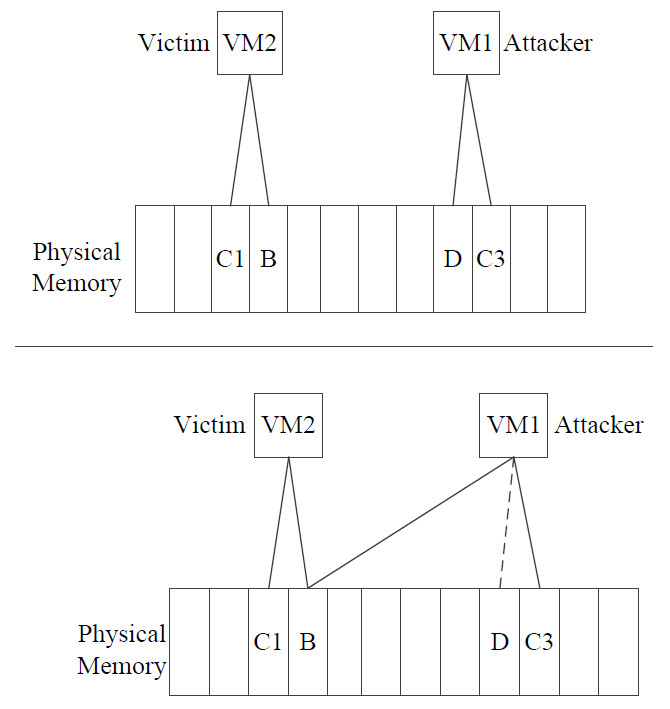
\includegraphics[width=8cm, height=7cm]{VMCS0.jpg}}%{pdfvmsm1.jpg}}
\caption{The execution process of double mapping. } \label{fig0}
\end{figure}

\textbf{Scene 2.}
    For the remapping attack, there are VM1 (attacker) and VM2 (victim). A physical page (named 'A') used by VM2 is released after being used. After 'A' is released, VM1 remaps to 'A'. So that the guest virtual address of VM1 points to the physical page 'A'. By this way, VM1 can access the information on 'A' used by VM2, causing information leakage.

Through the analysis of these two kinds of attack models, it is necessary to achieve attack prevention through VM monitoring and VM isolation.
\subsection{Assumption}

We propose some assumptions.
First, we assume hardware resources are trusted including processor, buses and so on, the trusted boot based on hardware can ensure the security and integrity of bootloaders. The TCB contains created HyperMI and hardware resources. Second, this paper does not consider denial of service attack (DOS), side channel attack and hardware-based attack, such as cold-boot attacks and RowHammer.


\section{Design}\label{sec:design}
In this section, we give an overview of HyperMI architecture.% and describe the three important modules.


\begin{figure}
\centerline{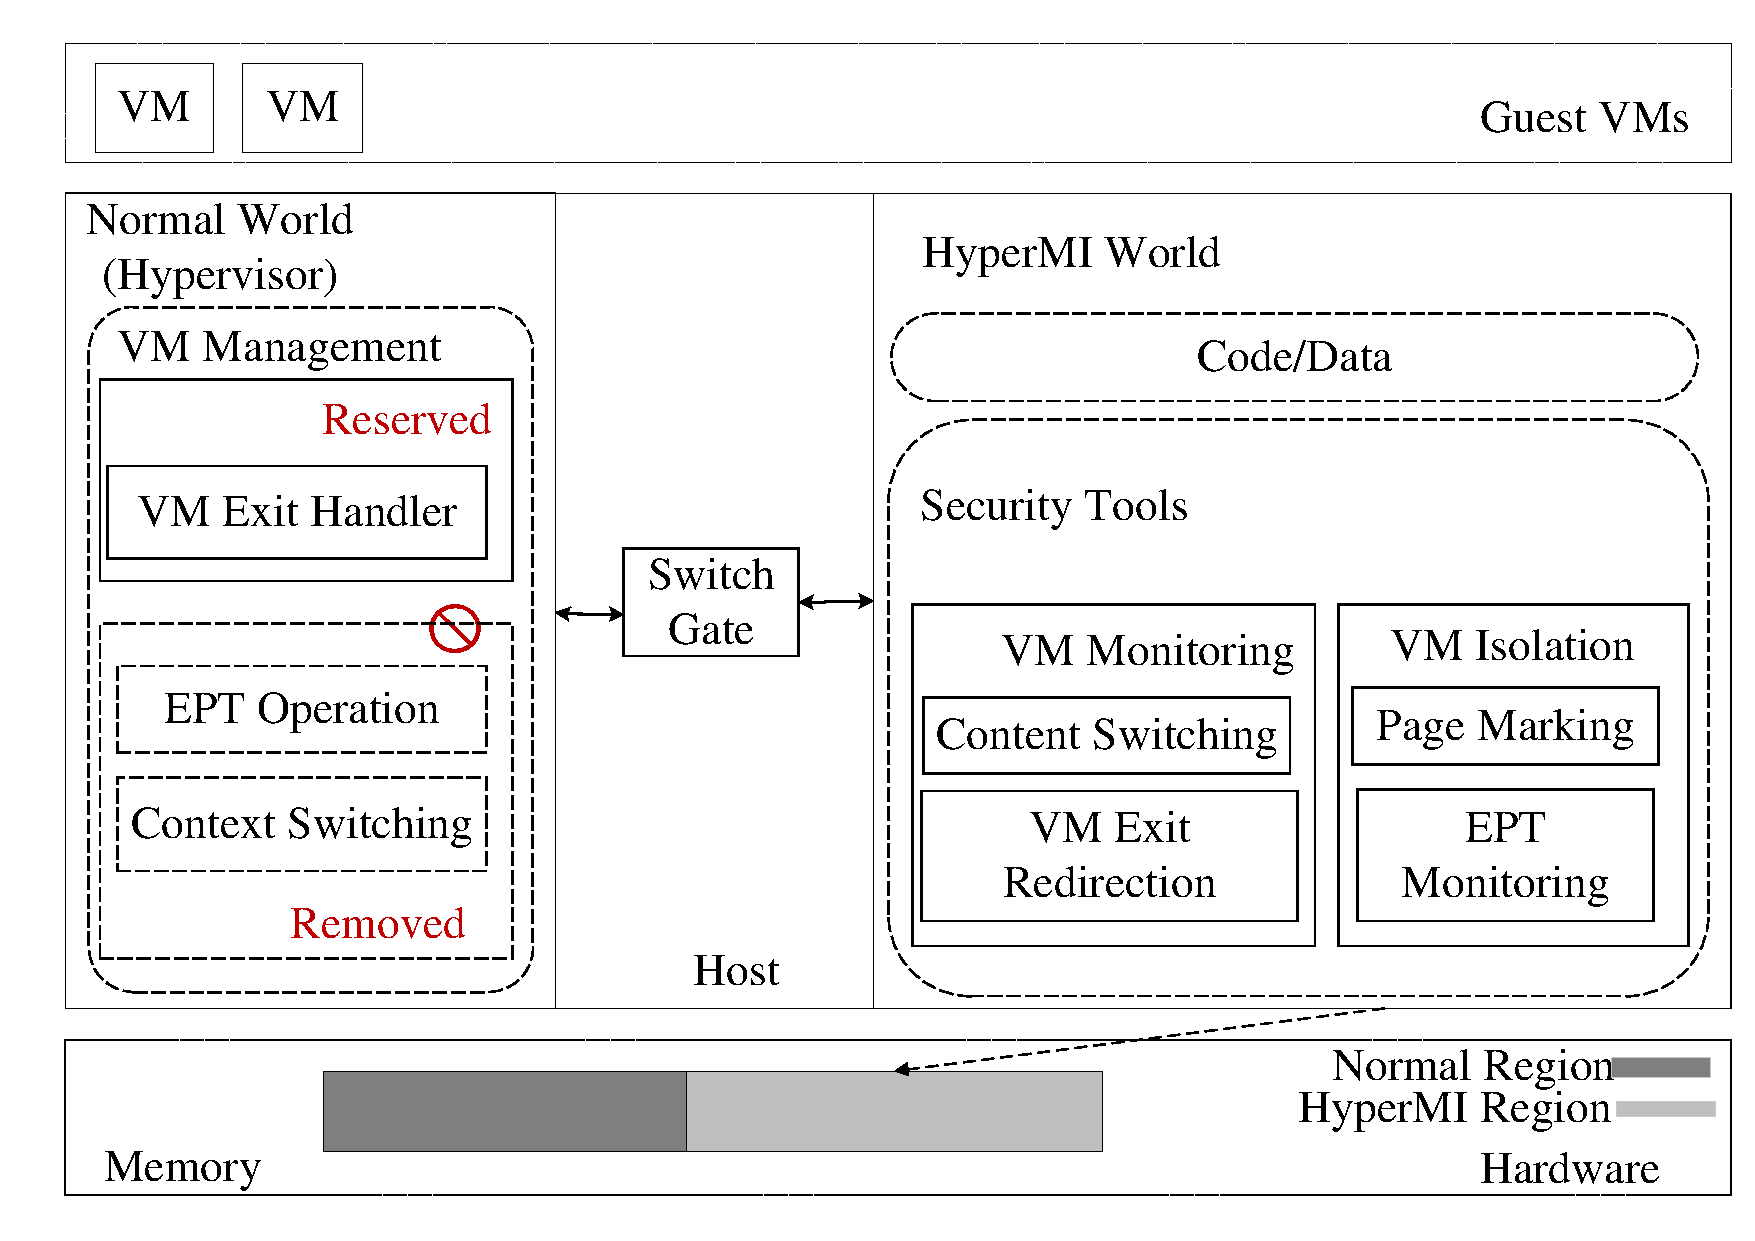
\includegraphics[width=9.5cm, height=7cm]{pdfvmcs1.pdf}}%{pdfvmsm1.jpg}}
\caption{The architecture of HyperMI. } \label{fig1}
\end{figure}

\subsection{Architecture} 
HyperMI is designed to provide a secure isolated execution environment to protect VMs against compromised hypervisor without depending on a higher privilege level software than hypervisor or extra customized hardware.



Figure \ref{fig1} depicts the architecture of HyperMI. The first component is the modified hypervisor, some functions such as EPT operations, context management, are stripped from the original hypervisor. Some functions that closely related to protected data structures are hooked, once these functions are called, the execution flow will be transferred to HyperMI world through Switch Gate. The second component is the HyperMI World, which is a secure and isolated execution environment based on the same privilege level with the hypervisor. VM Monitoring and VM Isolation, rely on this HyperMI world to ensure their security and isolation. The last component is the Switch Gate. This component is an atomic operation to ensure the secure switch between the normal world and the HyperMI world. 


While the hypervisor together with guest VMs run in the normal world, the hypervisor is forced to request HyperMI to perform four operations on its behalf: 1) switching context between the hypervisor and VMs, 2) updating EPT of VMs, 3) verifying the pages when executing swapping operations to resist double mapping attack, 4) verifying the pages when executing releasing operations to resist remapping attack. After setting up the HyperMI, the whole system is ready to create an isolated executing environment. With these designs, HyperMI enforces the isolation and protection of memory used by each VM. Furthermore, HyperMI guarantees the security of interaction, memory isolation between the hypervisor and VMs.

\begin{figure}
\centerline{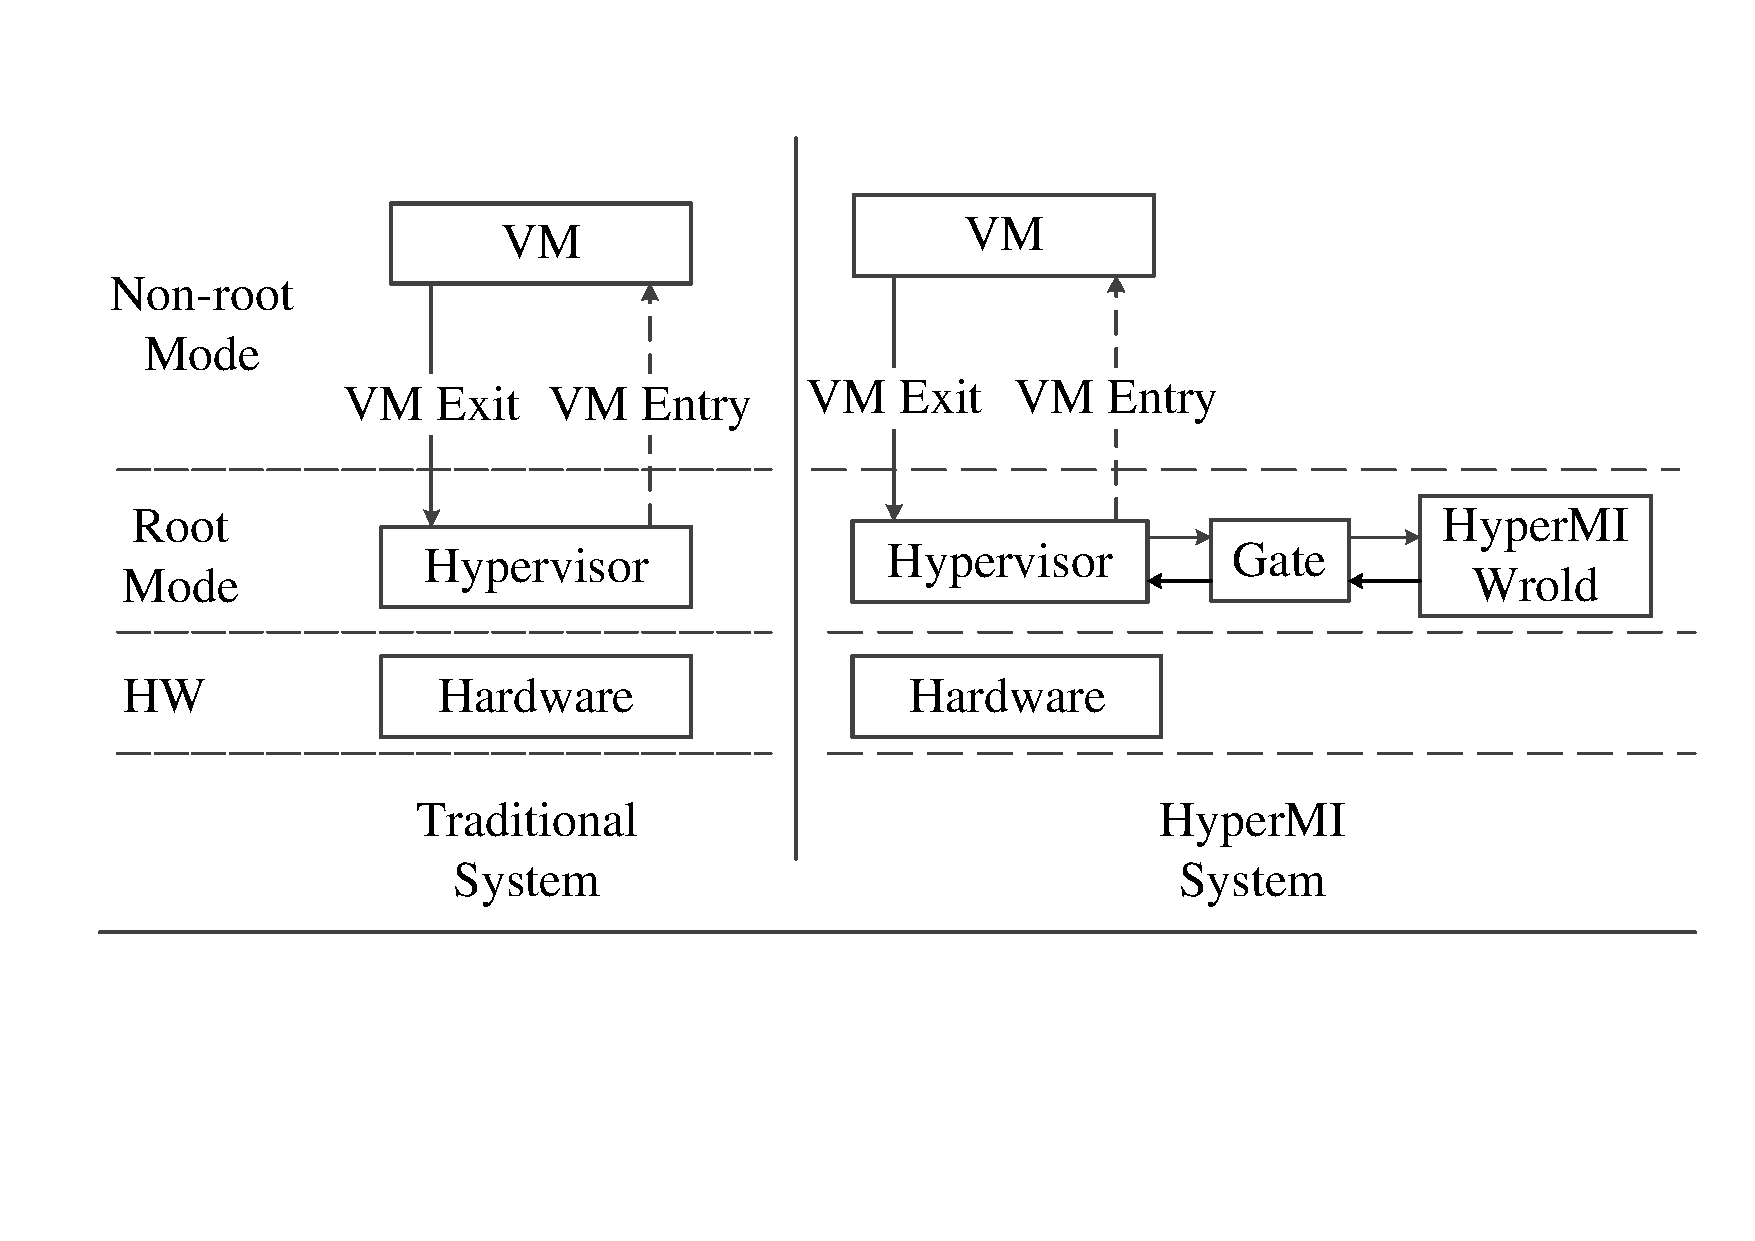
\includegraphics[width=9.5cm, height=7cm]{pdfvmcsProcess.pdf}}
\caption{Interaction comparision. } \label{fig+1}
\end{figure}

\subsection{Interaction} \label{IN}


Figure \ref{fig+1} shows the interaction process of HyperMI. 
As described in the previous architecture, HyperMI is placed at the same privilege-level with the hypervisor, but in different address space. The two worlds interact through the channel, switch gate.


In the original system, only guest VMs and the hypervisor are involved during the execution. In details, 1) The guest VM would deliver a trap or receive an exception to interact with the hypervisor. 2) On receiving the VM exit signal, CPU would change to root privilege from the non-root privilege. During this process, hardware would save all guest context to VMCS data structure automatically. 3) The context of the hypervisor, that is saved in VMCS too, would be loaded into registers. Then exit handler in the hypervisor gets to run. 4) The hypervisor would call VMRESUME instruction to return the control flow to the halted VM when exit handler is finished. The context of the guest VM stored in VMCS (the context may be modified by the hypervisor during this process) would be loaded into register. 5) The guest VM resumes to run.

In HyperMI system, HyperMI hooks all functions which are involved in the interaction between the guest VM and the hypervisor. Besides, functions that are involved with EPT operation are also hooked to provide protection to EPTs. Therefore, the execution flow during VM exit has been changed on introducing HyperMI. The first two steps of VM exit are the same with that of the original system. For the third step, because the VMCS is protected by HyperMI, and the compromised hypervisor could not access this data structure. Thus, at the time, the functions used to read or write VMCS in the compromised hypervisor would be hooked and be redirected to the HyperMI world, security checks would be performed to ensure the legal operation on them. It is the same with this process when functions that are involved with EPT are called. 
After the legal operations, HyperMI would transform control flow to the compromised hypervisor to perform VMRESUME. Because VMCS and EPT is perfectly isolated and secured from the compromised hypervisor, the compromised hypervisor cannot subvert guest VMs by modifying these two most crucial data structures.


\section{Implementation}\label{sec:imp}

HyperMI is implemented on x86 platform based on KVM.
We describe the implementation of key components in the HyperMI architecture below including HyperMI world, VM monitoring and VM isolation.

\subsection{HyperMI World} \label {HWorld}

\begin{figure}
\centerline{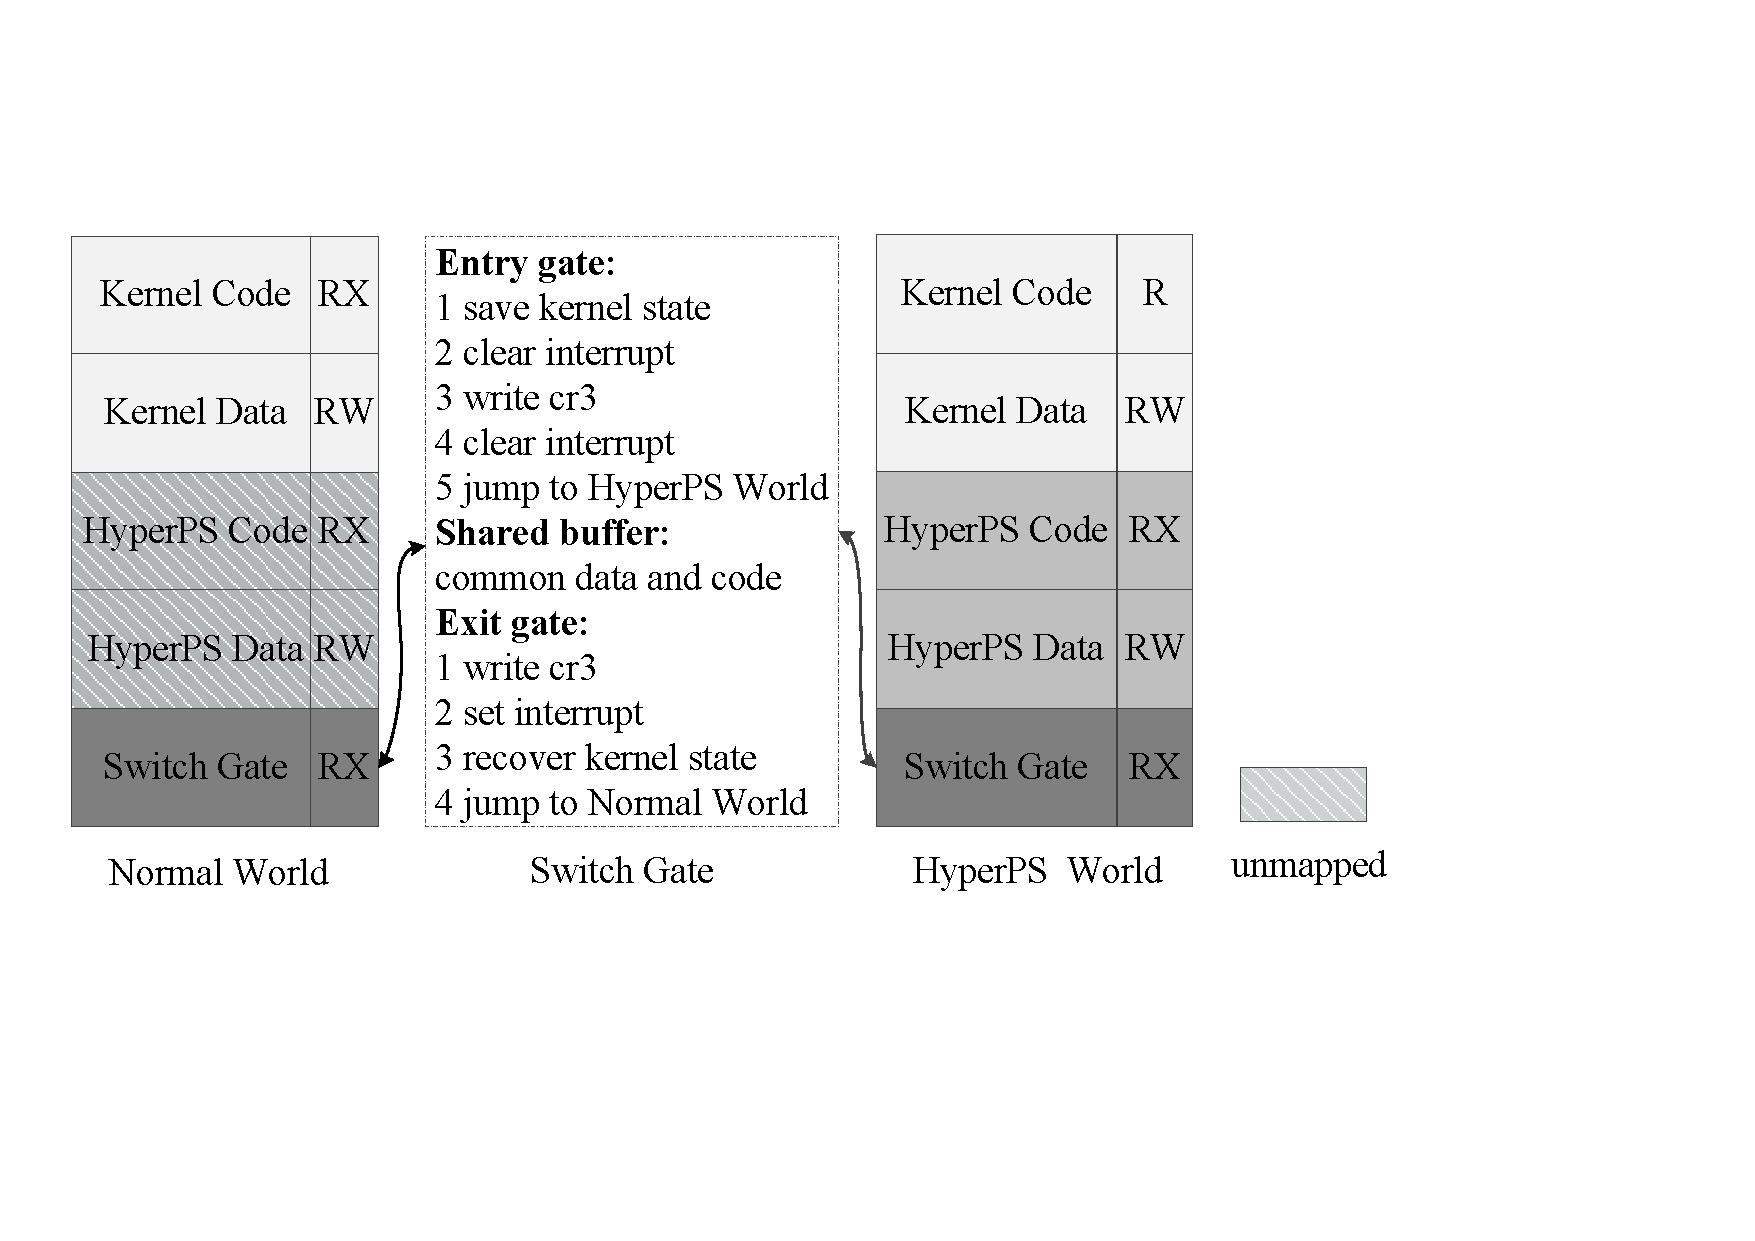
\includegraphics[width=11cm, height=8cm]{pdfvmcs2.pdf}}%{vmsm23.jpg}}
\caption{An overview of address space layout.} \label{fig2}
\end{figure}

HyperMI world, based on another kernel page table, is created to be another address space at the same privilege-level with hypervisor. %resist compromised hypervisor against leaking information, accessing data illegally and falsifying data. 
Switch gate is created to provide the only communication channel for two worlds.


\textbf{Creating HyperMI World}
%HyperMI world is created to provide a secure execution environment for security tools against compromised hypervisor. 
To satisfy isolation, the code and data segment of HyperMI world must not be accessed by normal world. We use two isolated address space based on two sets of page table to achieve isolation.
Figure \ref{fig2} describes the address space layout of two worlds through two sets of page table, the normal page table and HyperMI page table. On the left of Figure \ref{fig2}, the normal page table contains code and data of the normal world except for that of HyperMI world in case of compromised hypervisor breaking the integrity of HyperMI world. So that program running in normal world cannot access data in HyperMI world. On the right of Figure \ref{fig2}, all address are mapped in HyperMI page table.
HyperMI code remains executable and HyperMI data remains writable. What's the most important, kernel code is forbid to execute with reference to protection for running HyperMI world, so that non-executable kernel code  cannot attack HyperMI world.

\textbf{Creating Switch Gate}
In the middle of Figure \ref{fig2}, the switch gate includes entry/exit gate and shared buffer. Entry gate provides the only entrance to HyperMI world while the exit gate provides the address for returning to the normal world. The shared buffer contains common data and code which the system needs to run the switch process. Common code is switch code, common data is entrance address to the HyperMI world and return address to the normal world. The switch gate is mapped at the same place in the normal world and HyperMI world because the page table loading code must be called by the two worlds before and after switching. Of course, the entrance address must be protected after switching to HyperMI world in case of a malicious attacker accessing HyperMI world causally after trusted boot. This is introduced in section \ref{SG}.





\subsection{Security Guarantee for HyperMI World}\label {SG}
Nevertheless, without any protection measures, the page table to load to switch to HyperMI world is not secure for four reasons: 1)Attackers can control page table with the highest privilege after hypervisor is compromised. 2) Attackers can bypass the switch gate to break the security of HyperMI world. 3) Attackers with the highest privilege can free to execute privileged instructions to access the value of privilege registers, such as CR0, CR3 and so on. 4) Attackers can carry out DMA attack to access HyperMI world casually.
We detail the protection measures for these four types of attacks below.
%\paragraph


\textbf{Protecting Page Table}
Hypervisor has full control of page tables, so it can attack the HyperMI world which is based on page table.
% Actually, protection for page tables is detailed in section \ref{HWorld}. 
There are three reasons for controlling the two set of kernel page tables: 1) To access casually or bypass HyperMI world, the attacker can tamper the content of normal page table to map address of HyperMI world or load malicious page table to CR3.
%2) To execute code injection attack, the attacker can close the write protection mechanism by modifying the value of CR0 register, changing the access permission bits of the memory page. 
2) The attacker can cover the hooked functions which we use in VM monitoring, redirect the functions to their own malicious code and bypass secure monitoring of HyperMI. 3) To break HyperMI world, malicious kernel code with execution permission can be executed to subvert HyperMI world by means of the vulnerabilities of the original kernel code. 
%access HyperMI world causally when HyperMI world is running if kernel code has the execution permission. 
Therefore, three secure approaches against these attacks are as follow.

For the first attack, HyperMI code and data is unmapped in page table of normal world. And to protect the entrance address to HyperMI world from being leaked,
%pre-allocate some space during trusted boot which kernel can't access directly through MMU, critical data in
we remove all entries that map to HyperMI world from the page table in normal world. Deprive the ability to access CR3 of the kernel in order to avoid loading illegal page table, and resist bypassing HyperMI world.
For the second attack, we intercept the accessing operation to CR0 and maintain the WP bit as 1. We stick to W$\oplus${X} and maintain the code segment of hooked functions unwritable.
To go against the third attack, we set the kernel code segment as NX (non-executable) when HyperMI world is running. For more security, we modify the kernel to configure these two sets of page table as read-only by setting the memory regions of the page tables unwriteable. This is necessary to prevent the page tables from being modified by attackers. Any access permission modification to two sets of page table must cause the kernel to page fault, then we dispatch page fault to HyperMI world to verify the correctness of address mapping. 
This idea is adopted in SKEE\cite{Azab2016SKEE}.


\textbf{Worlds Switching Securely}
HyperMI creates a switch gate for switch between the normal world and HyperMI world by loading a page table of the next space into CR3. And we must ensure atomicity and security during the switching process.

The switching process described in Figure \ref{fig2} is as follow: 1) Save the kernel state to the stack including general registers and interrupt enable/disable status. 2) Clear the interrupt with the CLI instruction. 3) Load the page table to the register CR3 and flush the TLB. 4) Interrupt again. 5) Jump to the HyperMI region. For the exit process, return to the normal world by performing the operations in the reverse order.

If we don't use the switch process above, just write the address of different page tables to CR3. Switch to HyperMI world and return to normal world directly. Attackers can attack the system by violating security. Attackers can get the address of HyperMI world by accessing the register CR3. We use interruption policy (the first step) in our switching process to prevent this attack. 
If there is not the second interruption (the fourth step), attackers can implement another attack. They can jump the first interruption.
%and get the base address of page table of HyperMI world from CR3. 
Then they can access HyperMI world successfully. 
%This attack can go against security and atomicity.
However, we adopt twice interruption policy (the fourth step) in our switching process to prevent this. 
%Twice interruption is used to ensure security in case of attackers carrying out attack after the third step in our switch process. 
%After attackers jump the first interrupt and get the address from CR3, the second interruption can prevent attackers going to HyperMI world directly. 
This idea is inspired from the design of gate in SecPod\cite{Wang2015SecPod}.



\textbf{Accessing Privilege Registers Securely}
The hypervisor is still privileged and it can free to execute privilege instructions, so that it can write any value to the related privileged registers. 1) Malicious attackers can close DEP mechanism by writing to CR0, close SMEP mechanism by writing to CR4. 2) Kernel code can load a crafted page table to bypass the HyperMI world by converting a meticulously constructed address of one page table to CR3.
To protect the system, HyperMI deprives sensitive privileges instructions executed by the hypervisor, and dispatches the captured events to the HyperMI world. The HyperMI world can choose how to handle this event, such as issuing alerts, terminating the process, or doing nothing. The whole process is similar to the signal handling in traditional OSes.

\textbf{Resisting DMA Attack}
%Thirdly, it is important to focus on DMA attack. 
DMA operation is used by hardware devices to access physical address directly. Malicious attackers can read or write arbitrary memory regions including HyperMI world by DMA. Therefore, it is a crucial focus of intercepting direct access to physical pages belonging to HyperMI world by DMA operation. 
Fortunately, HyperMI employs IOMMU mechanism to avoid DMA attack, which can carry out access control for DMA access. Our approach adopts two policies: 1) Remove the corresponding mapping of the critical data from the page table which IOMMU uses. These critical unmapped data includes the entrance address of HyperMI, data recording Page-Mark structure used in VM isolation, VM-Mark structure used in VM monitoring and so on. 2) Intercept the address mapping functions about I/O, verify whether the address is an address space of HyperMI world, then choose to map or unmap.


Through the above security measures, HyperMI can be protected from being bypassed and being breaking, thus providing a secure execution environment for VM monitoring and VM isolation.














\iffalse
\begin{figure}
\centerline{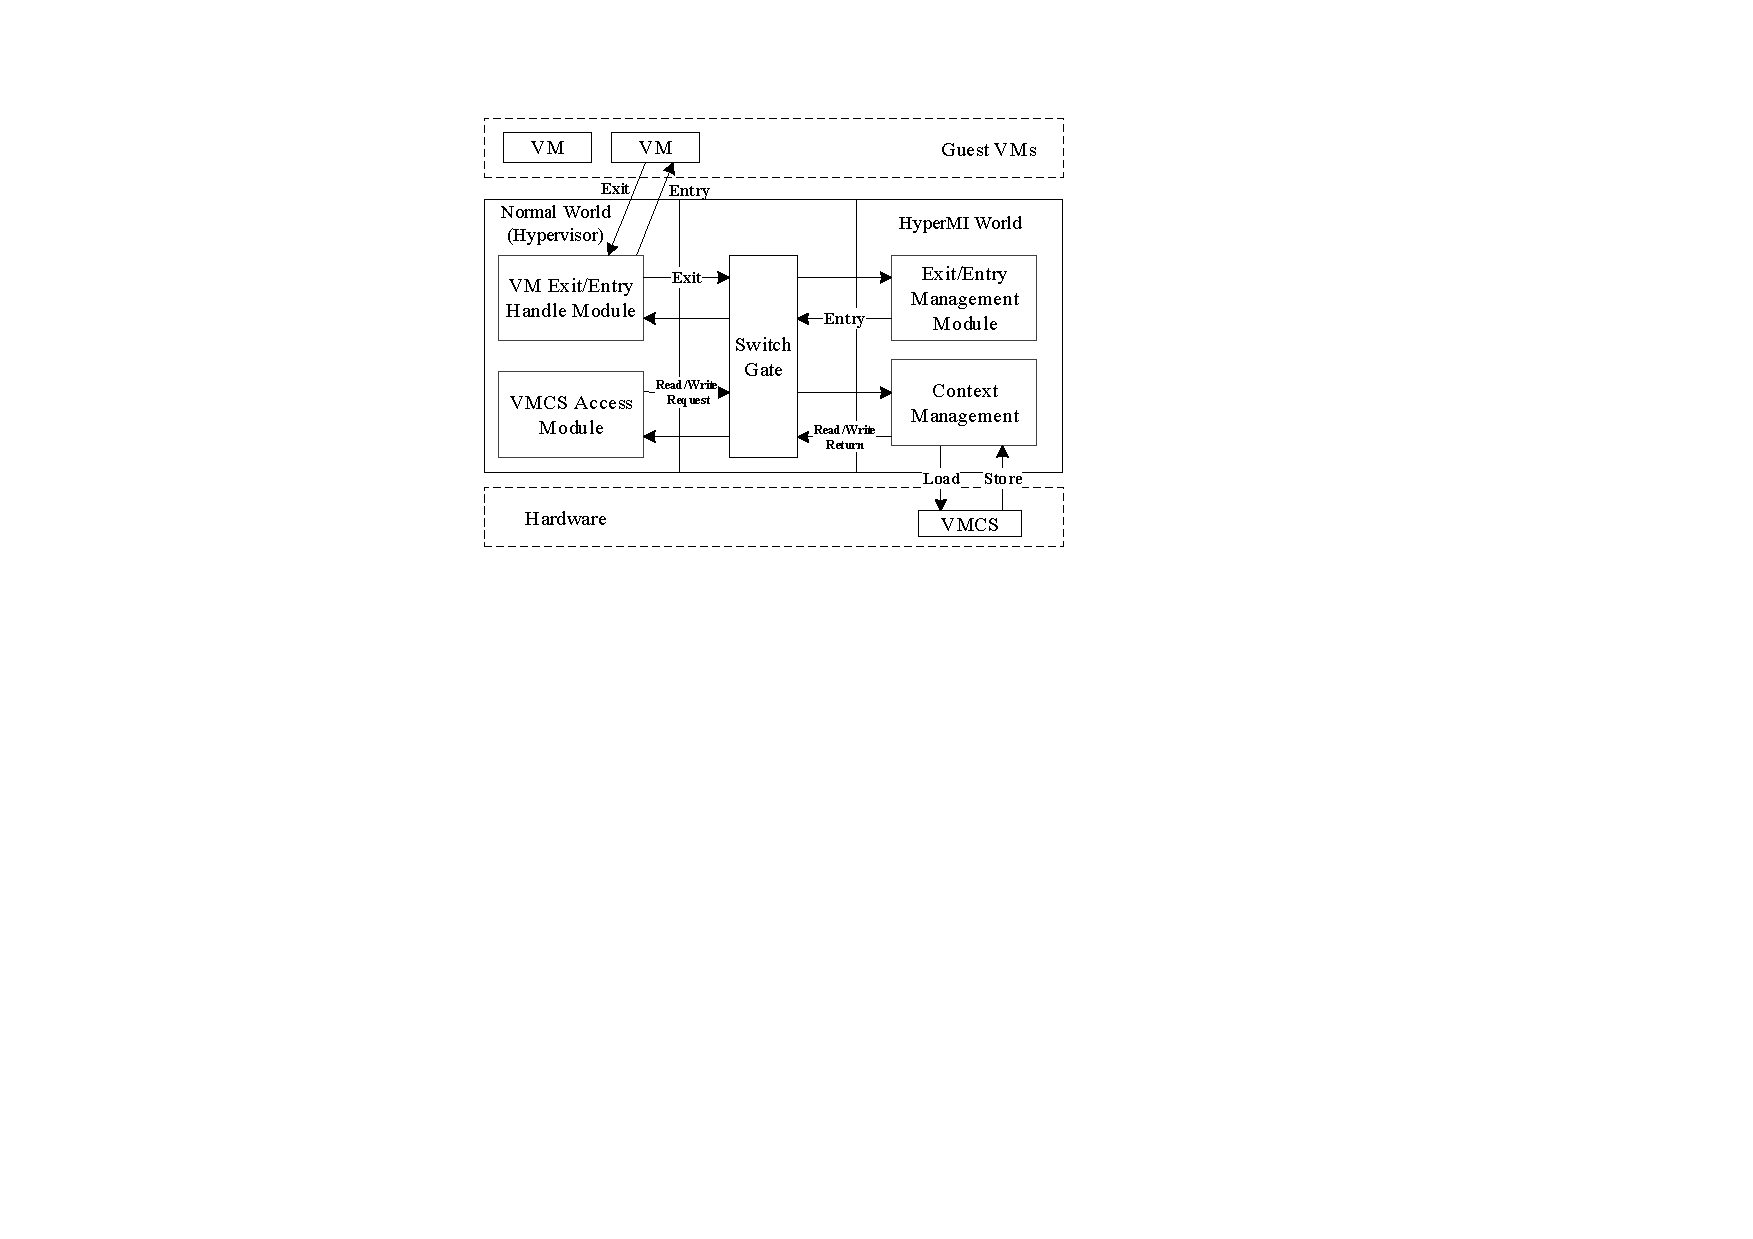
\includegraphics[width=9cm,height=6.5cm]{pdfvmcs4.pdf}}%{vmsm43.jpg}}
\caption{An overview of VM monitoring.} \label{fig4}
\end{figure}

\fi



\subsection{VM Monitoring}\label{vmmonitor}

During the VM entry/exit process, the related state information of every virtual CPU and host OS are stored in VMCS structure. 
Moreover, only the VMX root privilege instructions, such as VMPTRLD, VMPTRS, VMCLEAR, VMWRITE, and VMREAD, can operate the VMCS.
VM exit/entry are the points to intercept accessing operation of VMCS. HyperMI intercepts and validates interaction between hypervisor and VMs. Hypervisor needs to handle VM exit events according to different exit reasons during VM exit process while does not handle others during VM entry process. We describe two models: 1) Interception of context switching. 2) VM exit redirection.

\textbf{Interception of Context Switching}
The protection to VMCS structure cannot be ignored based on the fact that VMCS is structure recording all context information of the VM and it is managed by the compromised hypervisor. 
The VMCS structure always records the information of privileged registers, such as HOST\_CR3, EPT\_POINTER, HOST\_CR0, HOST\_CR4, VM\_EXIT\_MSR\_STORE\_ADDR, HOST\_RIP and so on. During the VM entry or VM exit, the compromised hypervisor can tamper VMCS structure, so that, the system can suffer these attacks: 1) Access memory region of VMCS directly. 2) Falsify the value of HOST\_RIP, and the system will suffer control flow hijack. 3) Tamper the value of EPT\_POINTER(EPTP), and another malicious EPT is loaded. 4) Fake the value of HOST\_CR3, so the page table of host OS can be replaced.

For the first kind of attack, to prevent compromised hypervisor accessing memory region of VMCS structure, HyperMI hides the base address of VMCS structure in HyperMI world. So, hypervisor loses the ability to access VMCS structure. In order to guarantee the normally running of original system, the hypervisor must require HyperMI to return the signal information rather than the real address on demand or trap the functions to the HyperMI world, and avoid many functions about VMCS operations to access the address of VMCS structure directly. To avoid the last kind of attack, in addition to hiding the address, HyperMI also intercepts and validates the execution of these instructions by placing hooks at these functions (vmcs\_writel, vmcs\_readl et al.). So hypervisor requests HyperMI world to handle operations about VMCS and return the corresponding result for the legal request. 


\textbf{VM Exit Redirection}
VMCS structure can only be accessed during VMX root operation. Therefore, the switching point between VMX Non-Root operation and VMX Root operation provide HyperMI a perfect point to perform the security check. In details, HyperMI would intercept and manage the process of VM Exit/Entry in HyperMI world to perform the security check for interaction data. 

As described in Section \ref{IN}, hypervisor needs to handle VM exit events according to different exit reasons during VM exit process while does not handle others during VM entry process. 
To handle VM exit events, HyperMI chooses a novel way.
Firstly, when VM exit happens, it finishes context management to provide security check for accessing interaction data (VMCS). Secondly, for subsequent VM exit events, it dispatches VM exit events to the hypervisor to handle. 
%especially, to cut down the performance overload, HyperMI set VM exit to configure of conditional exit events as non-running and reduce the occurrence number of exit events.



\subsection{VM Isolation}\label{VMISolation}


As known to all, when Intel VT-x is enabled, all the physical memory is managed by the hypervisor using Extended Page Tables (EPTs), EPTs must be involved in each memory access and determine the permissions of the accessed memory page frame. Besides, the hypervisor employs different EPTs to manage the corresponding physical memory area for different VMs. If the page is remapped or double mapped, the system causes a page fault. A VM accesses physical memory page frame through EPT updating. 
Page is accessed by VMs through EPT updating.
It is essential to control page mapping when EPT updates. To achieve the goal of VM isolation completely, we adopt page marking technique, that marks memory page with flag and tracks the page. However, a time point is needed for marking all page. And it is no doubt that EPT updating is an excellent point because hypervisor can manage all page mapping efficiently when EPT updates. Besides, EPT must be protected in case of data being leaked because EPT plays a vital role in address translation of VMs. So we describe VM isolation in these two aspects, EPT interception and memory isolation for VMs.







Confronting with these attacks, we can see that the ultimate purpose of attackers is to access the physical memory page frames of other VMs. HyperMI solves the issue using the following policies: 1) Hide the address of EPT and make it unmapped for the kernel in the normal world. 2) Intercept the related operations including EPT creating, loading, updating, walking and destroying to avoid leaking the address of EPT. 3) Mark respective EPT for every VM, isolate EPT among VMs, and ensure that the right and corresponding EPT is loaded for every VM.







\begin{table}[htbp]
\centering
\caption{VM-Mark Table.}\label{tab1}
%\begin{tabular}{c|c|c|c}
\begin{tabular}{p{1.4cm}|p{1.2cm}|p{1.1cm}|p{1.7cm}}
\hline
\multicolumn{4}{c}{\bfseries\textbf\centering{VM-Mark Table}}\\
\hline
{\itshape\bfseries Label} & VMID & EPTID & EPT\_Address\\
\hline
{\itshape\bfseries Description} & { The VM Identifier} & The EPT Identifier & The Entry Address of EPT\\
\hline
\end{tabular}
\end{table}

\begin{table}
\centering
\caption{Page-Mark Table.}\label{tab2}
%\begin{tabular}{|c{1cm}|c|c|}
\begin{tabular}{p{1.2cm}|p{1.4cm}|p{1.5cm}}
\hline
\multicolumn{3}{c}{\bfseries\textbf\centering{Page-Mark Table}}\\
\hline
{\itshape\bfseries Label} & OwnerID & Used \\
\hline
{\itshape\bfseries Description} & The Owner Identifier & Free or Used \\
\hline
\end{tabular}
\end{table}

For the first policy, three places should be particularly protected. The first place is the EPT creation function where the function would return a CR3-like address: EPTP value. The second place is VMCS where would record the value of corresponding EPTP. The last place is the hardware register EPTP, the work of this register is similar to that of the CR3 register, which is used to provide MMU with the location of EPT. 

\textbf{Interception of EPT Operations }
During the translation process of mapping GPA to HPA through EPT, a VM can suffer these attacks: 1) Compromised hypervisor can access EPT of every VM, then does whatever it wants by modifying the address mapping causing remapping and double mapping attack. 2) Load the malicious EPT and execute illegally.



Therefore, it is critical to intercept the EPT creating operation and protect the address of EPT in HyperMI world. Notably, it is vital to store VMCS structure which contains the value of EPTP in HyperMI world. 


%Specially, store VMCS structure including EPTP in HyperMI world. 
% However, some functions need the address of EPT to perform.
However, some functions, in addition to the EPT creation function, still rely on the value of EPTP. In this paper, HyperMI provides a novel approach that HyperMI returns signal information necessarily to these functions rather than a true address to make the system run normally. 



% There is a novel idea that HyperMI returns signal information necessarily to these functions rather than true address to make the system run normally.
For the second policy, some functions, EPT creating, loading, walking and destroying, need access address of EPT. HyperMI places hooks on these functions, then dispatch them to HyperMI world and handle appropriately. In the meantime, HyperMI handles double mapping to ensure that there is only one virtual address mapping to one physical memory page during the EPT updating, and handles remapping problems to ensure the content of page cleaned after page being swapped out. This will be described in detail later.



For the last one, intercepting the loading EPT operation and verifying the correctness of EPT can avoid loading a wrong EPT and leaking the content of physical memory page. To ensure one EPT for one VM, HyperMI creates the VM-Mark structure stored in HyperMI world as Table 1 described, and record VMID, EPTID, EPT\_Address and binds them together. VMID is created and destroyed based on hash value of the image of VM. EPTID and EPT\_Address is recorded as long as the EPT of current VM is created.




\begin{figure}
\centerline{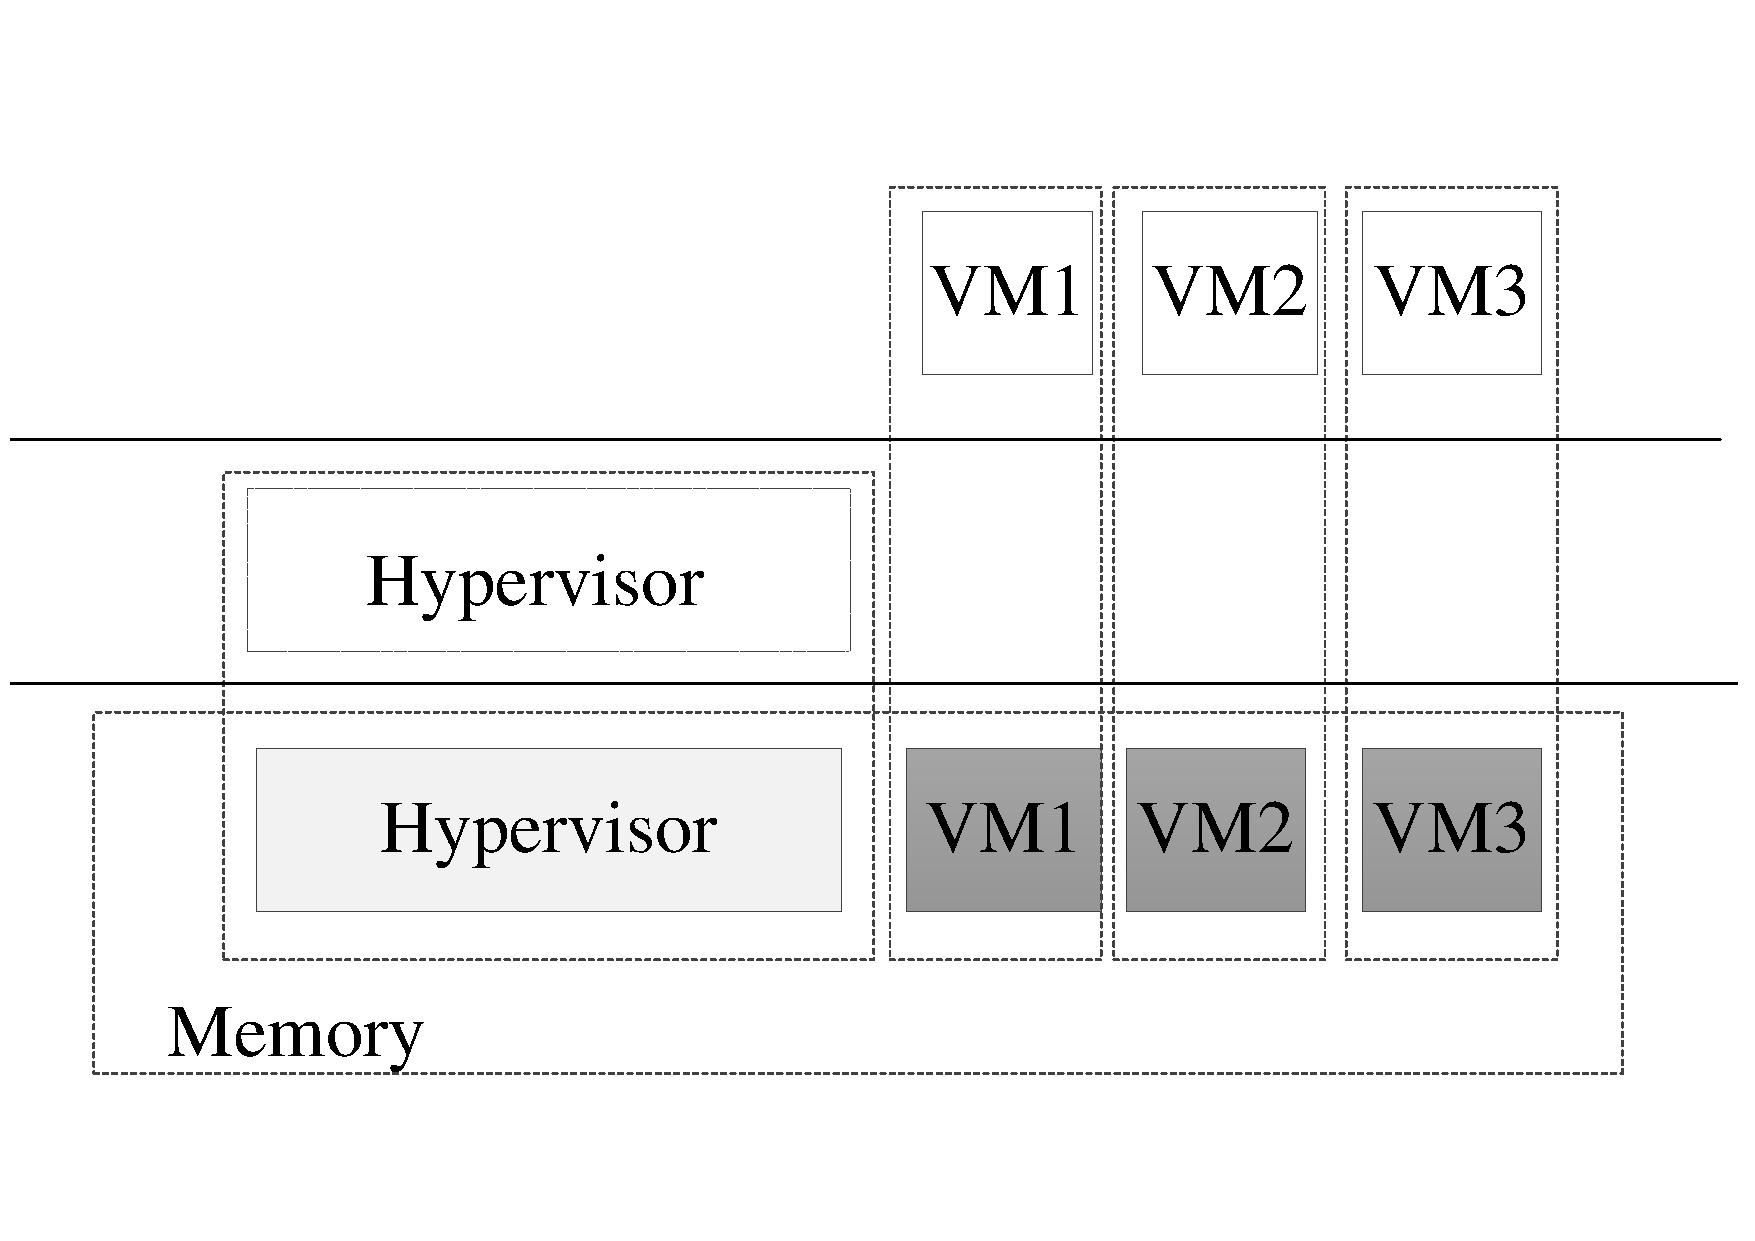
\includegraphics[width=9cm, height=6cm]{pdfvmcs3.pdf}}%{vmsm32.jpg}}
\caption{Memory isolation for VMs.} \label{fig3}
\end{figure}


\textbf{Memory Isolation for VMs }
% Besides isolated EPT above, it should be considered that isolate memory to achieve the goal of VM isolation completely, as Figure \ref{fig3} describes. Hypervisor and every VM just can access own physical memory. Without memory isolation mechanism, compromised hypervisor and compromised VM can access memory pages of victimized VM by two ways when EPT updates: 1) Double mapping. 2) Remapping to pages with content. So some efforts are done. Monitor EPT updating and create Page-Mark structure described in Table 2 to record the owner of every physical memory page.
In addition, the isolation EPTs mentioned above, isolating memory is another aspect that should be considered to achieve the goal of VM isolation completely, which is depicted in Figure \ref{fig3}. 
% Besides isolated EPT above, it should be considered that isolate memory to achieve the goal of VM isolation completely, as Figure \ref{fig3} describes.
Hypervisor and every VM can access own physical memory. Without memory isolation mechanism, compromised hypervisor and the compromised VM can access memory pages of the victimized VM by two ways when EPT updates: 1) Double mapping. 2) Remapping to pages with content. So some efforts are done. Monitoring EPT updating and creating Page-Mark structure described in Table 2 to record the owner of every physical memory page. 



In order to against the double mapping attack in the process of EPT updating, HyperMI should finish these two tasks: verifying the owner of pages firstly, and then marking the OwnerID of Page-Mark structure for unused pages or thwart the mapping operation for used pages in case of malicious double mapping behavior. So the technique of pages allocation can divide all the pages into different catalogs: the pages of hypervisor or the pages of every VM.

To go against the remapping attack, HyperMI cleans the context of the page when the page is swapped out, so attackers can't get the context of the page by the way of remapping. And HyperMI clears the Page-Mark structure of the corresponding page. This solution is the same as the treatment method of the pointer for the purpose of security protection. 



\section{Evaluation}\label{sec:evaluation}
We describe the design and implementation of HyperMI. In this section, we evaluate the protection effectiveness
and performance of HyperMI by exploiting vulnerabilities and comparing it with traditional KVM through a set of benchmarks.





\subsection{Security Analysis}


%new new111111111111


%In this paper, we propose HyperMI world, a secure isolation execution environment, which is located at the same privilege-level with the hypervisor. 
%We elaborate on the security and isolation of HyperMI world in the section \ref{HWorld}. 
%Actually, interaction security between VM and hypervisor, as well as memory isolation among VMs, is the most essential feature of HyperMI world.
%Similarly, the security of HyperMI World implemented by software methods also needs to be guaranteed.
% The security of the conception of same-privilege-level, has been fully elaborated in SKEE. 


HyperMI mainly provides three functions, HyperMI World is used to provide a secure execution environment to ensure the security of HyperMI itself, VM Monitor and VM Isolation are used to ensure the security of the upper virtual machine. VM Monitor is used to ensure the interaction security between VM and hypervisor and the running state security of VM. VM Isolation is used to ensure the memory isolation among VMs. Just as the threat model described in the section \ref{threat}, an attacker could subvert the upper guest virtual machines 
%in two ways: subverting the VM through a compromised hypervisor directly, or 
by implementing attacks such as cross-domain attack through a malicious virtual machine.
In this section, we will focus on how to achieve secure VM monitoring for interaction-data and secure VM isolation for memory among VMs, then describe protection for HyperMI against compromised hypervisor. Table \ref{tab3} shows the real attack instances in line with the above attack model. 

%However, these two attack vectors, regardless of their attack path, both focus on critical interaction data and data on memory, afterwards, modifying more detailed data, such as the VMCS data structure, EPT and EPT Pointer. Thus, we will elaborate on how HyperMI fends of these attack, and Table \ref{tab3} shows the two real attack instances in line with the above attack model. 
% the attack instances listed in Table \ref{tab3} perfectly match the description of attacker, so we will use these two instances to specifically analyze security performance. 


\textbf{Modifying Interaction-Data Attack}
We clarify interaction data including VMCS in Section \ref{vmmonitor}. VMCS mainly stores the context information of VM and host in VMX operation, such as control registers. To prevent interaction-data leakage, we protect VMCS from the attacker. Firstly, VMCS is hidden in HyperMI World and can not be accessed by hypervisor. Secondly, functions that can access VMCS address are hooked to Hyper World in order to avoid exposing VMCS address. The attacker can not get addresses and access VMCS, this prevents attackers from tampering with interactive data attacks. We implement corresponding attack cases (Interaction-data Attack) described in Table \ref{tab3}, mainly direct access to GUEST\_CR3 in VMCS. The experimental results show that the access failed, malicious interaction-data accessing is prevented successfully. According to the above analysis, the attacker can not access VMCS, and can not further attack. Therefore, the VM runtime states and interaction-data cannot be modified. 


%CVE-2009-2287 allows attacker to provide invalid value of CR3, which is an important data value in VMCS data structure. Because HyperMI would check the value of CR3 before VM entry instruction is conducted, an attacker has no chance to load the value to physical CR3 register successfully. HyperMI protects all important data values in VMCS data structure. In details, interaction between hypervisor and VMs runs in HyperMI world, VMCS structure used to record context switching data is hidden in HyperMI world, so an attacker cannot modify VM states during context switching. HyperMI adopts VM-Mark table to ensure that load consistent EPT for every VM, so attacker cannot modify EPTP. Therefore, the VM states cannot be modified. 




\textbf{Subverting Memory Across VMs Attack}
%A kind of attack is subverting memory protection across VMs. 
Original hypervisor manages the memory of VM through EPT which controls the address translation of VM, so compromised hypervisor can incur malicious memory access attack, such as double mapping attack and remapping attack. However, HyperMI hides the address of EPT in HyperMI World and hooks all operations about EPT into HyperMI World. Page tracking technology can make and prevents double mapping and remapping attack. Page tracking technology can ensure that each physical page has only one owner, verify the ownership of each physical page when EPT updates the mapping, and ensure the safe mapping of physical memory. Page Release Clearance technology can clear the contents of pages when they are completely released, ensuring information security.
%
The main attacks that attackers can execute on subverting memory are double mapping attacks and remapping attacks.
Firstly, double mapping happens when assigning memory pages that have already been owned by a hostile VM to a victim VM. Page tracking and write-protection of EPT prevents this kind of attack. For each new mapping to a VM, HyperMI validates whether the page is already in use. Meanwhile, the allocated pages must be marked in the Page-Mark table for tracking. Secondly, another challenge is page remapping attack by a compromised hypervisor from a victim VM to a conspiratorial VM. This attack involves remapping a private page to a different address space. To defeat this type of attack, HyperMI ensures that whenever an page is released, its content must be zeroed out before creating a new mapping.
We implement a real attack, CVE-2017-8106 in kernel version 3.12. A privileged KVM guest OS user accesses EPT, conduct attack via a single-context INVEPT instruction with a NULL EPT Pointer.Attackers can not implement successfully and incur EPT access fault because HyperMI hides the address of EPT in HyperMI World and hijacks the loading of EPT. Therefore, HyperMI can avoid subverting memory across VMs including double mapping attack, remapping attack as well as malicious EPT access.
% attacker is unable to subvert the upper VMs by exploiting the hypervisor vulnerability. 
%But an attack on memory is not limited to loading malicious EPT Pointer.


\begin{table}
\centering
\caption{Hypervisor Attacks Against HyperMI.}\label{tab3}
\begin{tabular}{p{2.8cm}|p{5.5cm}}
\hline
{\itshape\bfseries Attack} & {\itshape\bfseries Description} \\
\hline
Interaction-data Attack & Load a crafted GUEST\_CR3 value\\
\hline
CVE-2017-8106 & Load a crafted EPT value \\
\hline
DMA Attack & Access HyperMI world by DMA \\
\hline
Code Injection Attack & Inject code and cover hooked functions to bypass HyperMI world \\
\hline
\end{tabular}
\end{table}

\textbf{Destroy HyperMI World}
HyperMI is created by relying on page tables. When HyperMI does not work, the original kernel with high privileges can access any page tables and modify them. It can also access control registers casually, redirect hooked functions used to monitor previously, and even maliciously destroy HyperMI World through DMA. We analyze the protection of HyperMI World from these four aspects, page table modifying attack, hooks redirection attack, reg attack and DMA attack.

\subsubsection{Page Table Modifying Attack}

Page table protection has been introduced in section \ref{SG}. The entry address mapping of the new page table is deleted from the old page table mapping to prevent the kernel from accessing HyperMI World directly through the page table mapping. When HyperMI World is active, the kernel code does not have any executable permissions in case of attacking running processes in HyperMI World. An attacker may attack in two ways.
First, the attacker may try to directly access the new page table address on the kernel page table by virtual address mapping, but when he accesses it, there is page fault due to the absence of address mapping.
Moreover, the attacker may run kernel code while the HyperMI World is active to attack programs running in the HyperMI World. This can be prevented because of the absence of executable privilege of kernel.


\subsubsection{Hooks Redirection Attack}

Due to the code of hooked functions including VMCS operations, EPT operations and  control register access operations is writable-protection, CR0 register access operation used to set W$\oplus${X} is controlled and page table updating used to change code execution privilege is limited, the attacker can not redirect hooked functions and bypass being monitoring.

\subsubsection{Reg Attack}

Access to some registers access operations including CR0, CR3, CR4 are controlled and hooked to HyperMI World. CR0 register can control the W$\oplus${X} privilege of code, CR3 can control the loading of page table and CR4 can decide SMEP mechanism. Protection for page table, hooked functions and regs play a role mutually in protection for HyperMI. 

\subsubsection{DMA Attack}

In addition, the memory can be accessed through DMA operations bypassing the MMU, except for accesses by executing memory accessing instructions. DMA attack is described in detail in section \ref{SG}. Attackers can use this feature to read or corrupt arbitrary memory regions. DMA attacks are not a threat to HyperMI, because HyperMI is inherently secure against DMA using IOMMU. Remove the corresponding mapping of the critical data from the page table which IOMMU uses. These critical unmapped data includes the entrance address of HyperMI, data recording Page-Mark structure used in VM isolation, VM-Mark structure used in VM monitoring and so on. DMA attacks that aim at modifying the VM memory or the page tables will also be defeated.



\subsection{Performance Evaluation}

In HyperMI, the kernel is modified so that the HyperMI World is initialized during the boot up sequence. This includes creating a new memory page table for HyperMI, allocating memory pages, as well as creating Page-Mark table and VM-Mark table. This process introduces security verification for pages according Page-Mark table, and security accessing for VMCS in HyperMI World during VM Exit/Entry sequence.

The kernel is modified to place hooks upon some control registers, accessing VMCS operations, and accessing EPT operations。
% in order to achieve HyperMI World, VM Monitoring and VM Isolation.
 The hooks jump to HyperMI World through the switch gate. So HyperMI can introduce some world switching overhead using switch gate.

We do not directly compare HyperMI with previous software approaches, as they cannot support all functions simultaneously. In order to assess the effectiveness of all aspects of HyperMI, we conduct a set of experiments to evaluate the performance impact imposed by HyperMI against an original KVM system (the baseline). We run three groups of experiments and compare the performance overhead, benchmarks performance overhead, VM load time as well as VM Exit/Entry overhead.
%. 
For simplicity, we only present the performance evaluation on a server with 64 cores and 32 GB memory, running at 2.0 GHz. Different experiments are based on different guest VMs. Both the original and HyperMI systems have the same configuration except the protection supported by HyperMI. The deviation of these experiments is insignificant. All the experiments are replicated fifty times and the average results are reported here.

\begin{figure}
\centerline{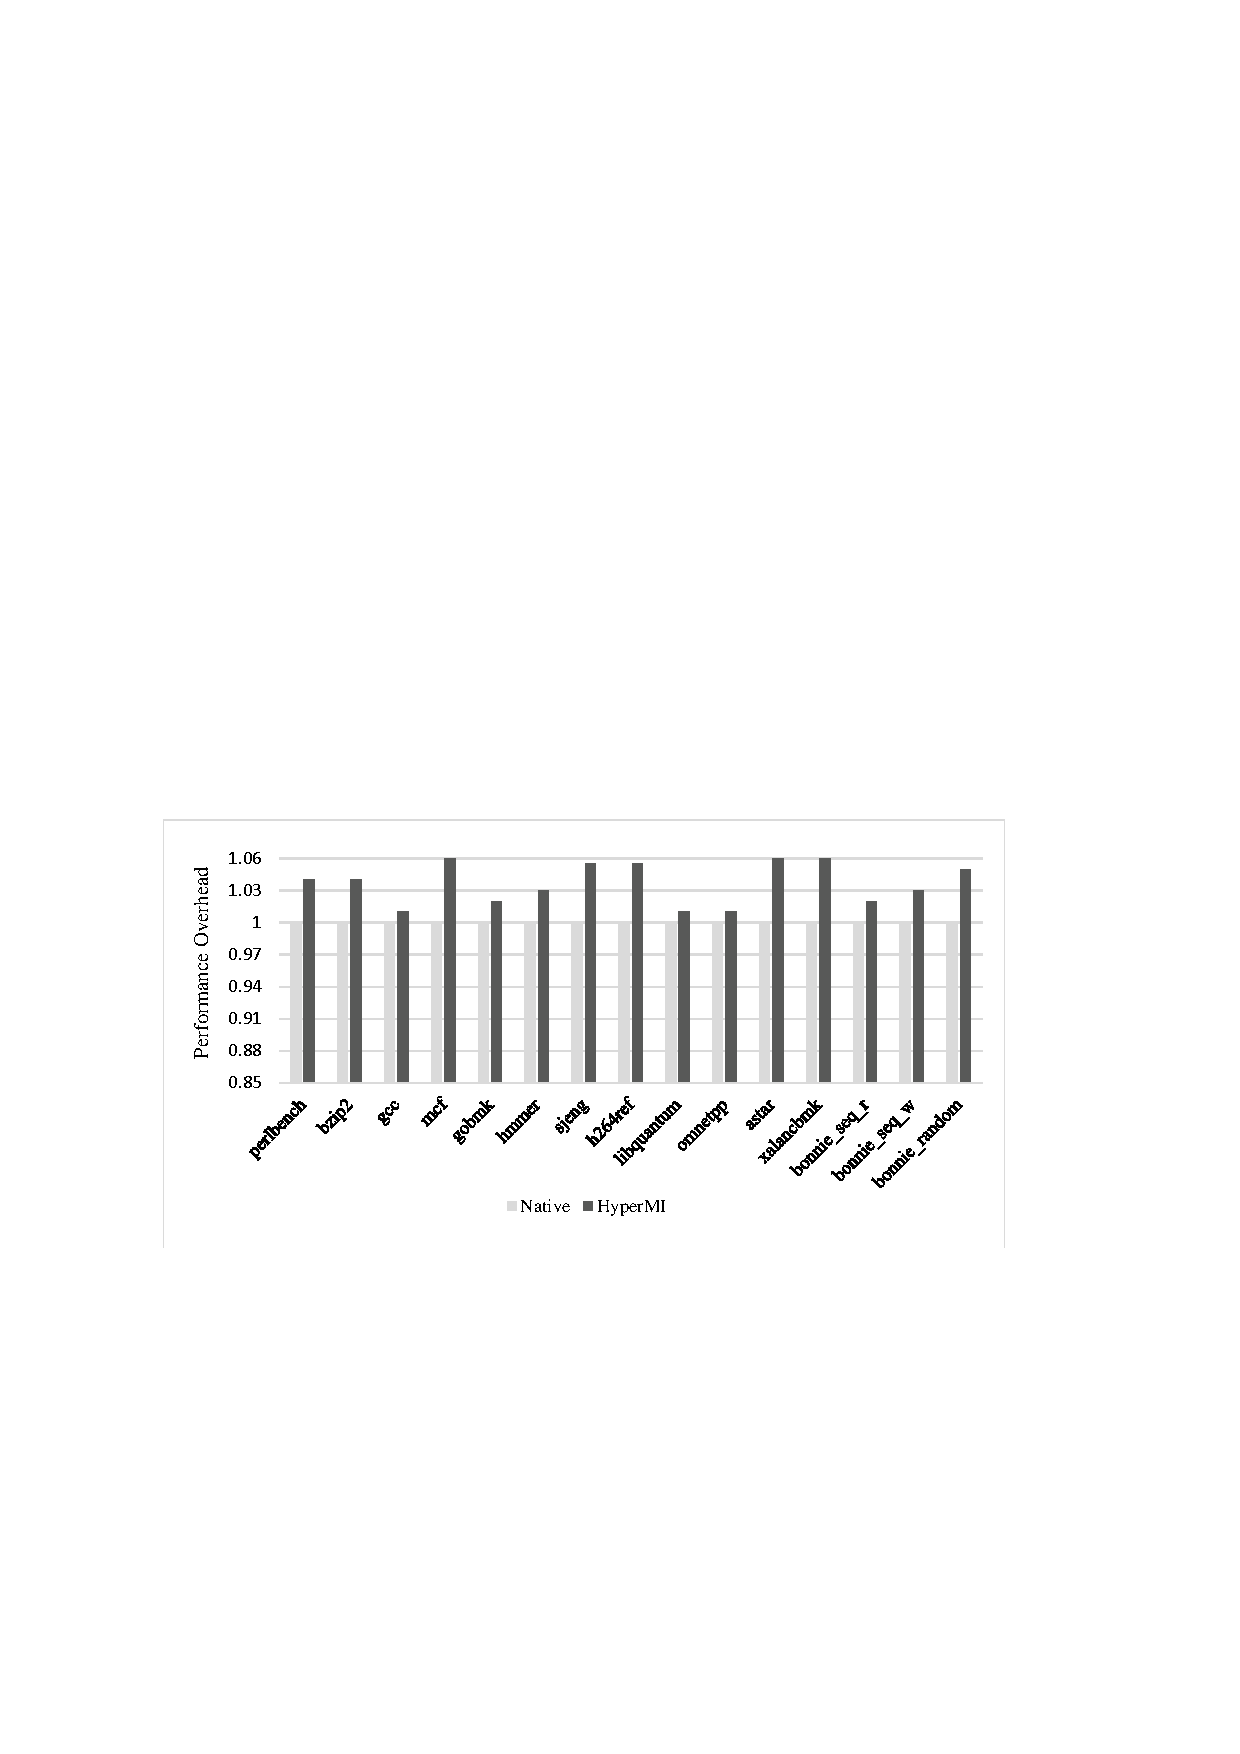
\includegraphics[width=9cm,height=5.5cm]{performance.pdf}}
\caption{Performance overhead.} \label{fig5}
\end{figure}

\textbf{Benchmarks Performance}
%All experiments are done on a server with 64 cores and 32 GB memory, running at 2.0 GHz and 5 VMs. 
In order to obtain the impact of HyperMI to the whole system, we measure HyperMI with microbenchmarks and application benchmarks. 
The version of hypervisor KVM is 4.4.1. We use one guest VM, the guest VM is with Linux kernel 4.4.1 and configured with 2 virtual cores and 2 GB memory. 
%All experiments are done 50 times and results are from the average.

To better understand the factor causing the performance overhead, we experiment with compute-bound benchmark (SPEC CPU2006 suite) and one I/O-bound benchmark (Bonnie++) running upon original KVM and HyperMI in a Linux VM. The experiments result described in Figure \ref{fig5}(the last three groups) shows relatively low cost. Most of the SPEC CPU2006 benchmarks (the first twelve groups) show less than 6\% performance overhead. It's not surprising as there are few OS interactions and these tests are compute-bound. Mcf, astar, and xalancbmk with the highest performance loss allocate lots of memory, and HyperMI handles Page-Mark structure and verify legality of page mapping when EPT updates. This can incur worlds switching which involves control register access and incur VM exit which involves page fault of EPT.
% and fewer TLB flushes with PCID technique because the two worlds are at the same privileged layer.
 For Bonnie++, we choose a 1000 MB file to perform the sequential read, write and random access. The performance loss of sequential read, write and random access is 2\%, 3\% and 5\%, not high, the main reason is that HyperMI has no extra memory operations for I/O data. The performance result shows that HyperMI introduces trivial switch overhead of two worlds and trivial overhead of memory isolation of VMs.

\textbf {VM Load Time}
% and World Switch Overhead}
The load time of a VM is a critical aspect of performance, because it influences user experience. We organize experiments to evaluate the performance impact of HyperMI prototype for a VM loading. Experiments are done with 4 VMs, each guest VM is with Linux kernel 4.4.1, configured with 2 virtual cores, and memory sizes from 512MB to 4GB.
 As expected, the VM booting time in HyperMI increases as the memory sizes increase, and the growth amplitude is more and more larger due to the world switch and page tracking caused by frequent memory allocation. We also measure the impact of completely booting a VM (configured with 2 VCPU and 512MB memory). As the result shown, the booting time is suffered a 2.3 times slowdown under HyperMI, due to the extra overhead of worlds switching and Page-Mark table accessing. Such overhead is worth for HyperMI.

\textbf {VM Exit/Entry Overhead}
Experiments are done on one VM with Linux kernel 4.4.1 and configured with 2 virtual cores and 2G memory. Network accessing can introduce lots of VM Exit, afterwards VMCS accessing in HyperMI World and world switches. In order to measure the performance impact of HyperMI, we use Netperf (version 2.7.0), a benchmark for measuring various aspects of networking performance, to determine VM Exit/Entry performance overhead. We run a netperf process in the tested VM, sending TCP or UDP streams under different load. The performance of I/O instruction exits (i.e., VM exits triggered by the guest's I/O requests) is shown in Table. 6. When we send or receive 1024-byte packets to or from an external server, HyperMI introduces xxx times VM Exit per second, xxx\% less than original KVM. Based on experimental results, we conclude that VMCS accessing in HyperMI World and worlds switching can be accepted.



\section{Related work}\label{sec:related}
We describe the related work from these four aspects, integrity verification for hypervisor, reconstructed hypervisor, customized hardware, and the same privilege level isolation. The first aspect is considered from the perspective of protecting the hypervisor, and the other three aspects are considered from the perspective of protecting VMs.

%\subsection{Protection for Hypervisor}

\subsection{Integrity Verification for Hypervisor}
In order to ensure the security of the hypervisor during trusted boot and runtime, an effective and commonly used method is to verify the integrity of the hypervisor, and reduce the attack surface. For the security of the hypervisor during trusted boot, paper \cite{Petroni2007Automated} proposes control flow integrity protection policy, by verifying regularly control flow integrity behavior to detect rootkit attacks. However, attacker can detect the regular and bypass the detection. For runtime security of the hypervisor, HyperSafe \cite{Wang2010HyperSafe} and HyperCheck \cite{Wang2010HyperCheck} choose pooling-query method based on SMM to finish integrity verification of hypervisor. However, SMM doesn't support for MMU. And attackers can hide trace during polling-query intervals when comparing to event-driven monitoring.

%\subsection{Resource Isolation}

\subsection{Customized Hardware }
Some works at the hardware level complete the protection of the process by extending the virtualization capabilities. These tasks provide fine-grained isolation of processes and modules from the hardware level. Haven \cite{haven} uses Intel SGX\cite{Hoekstra13cuvillo,Mckeen2013Innovative} to isolate cloud services from other services and prevent cross-domain access. SGX provides fine-grained protection at the application space instead of hypervisor space, and needs developers spend time reconstructing code and dividing code into trusted part or untrusted part. SGX has requirement for version of CPU. The effort \cite{Cho2016Hardware} combines the advantages of ARM TrustZone and virtualization to improve system performance, and isolate critical process components securely and efficiently. H-SVM\cite{Jin2015H} utilizes the hardware extension features of the CPU, and extends SMM microcode to achieve memory resource isolation among virtual machines. It deprives ability of accessing to memory resource by replacing the source code of the original hypervisor to access memory resource. Vigilare\cite{Moon2012Vigilare} and KI-Mon \cite{Lee2013KI} provide monitoring for access operations by introducing extra hardware. Vigilare provides a kernel integrity monitor that is architected to snoop the bus traffic of the host system from a separate independent hardware. It adds extra Snooper hardware connections module to the host system for bus snooping. KI-Mon monitors write operation to system bus and handles data to write in order to check rootkit attack.
%However, for cloud providers, these approaches means high-cost and low practicality as long as they are carried out widely.
%KI-Mon monitors write operation on system bus and handles data to write in order to check rootkit attack.

\subsection{Reconstructed Hypervisor }
Except for approaches based on hardware, some works\cite{nexen,Steinberg2010NOVA,hyperlock} pay attention to software isolation. Pre-allocating physical resource and completed isolated environment for every VM can avoid VM cross-domain attack, and data leaking attack. NOVA\cite{Steinberg2010NOVA} divides hypervisor into micro-hypervisor and user hypervisor running in root mode, adopts an idea which is similar to fault domain isolation to guarantee an isolated user hypervisor for every VM. The drawback of this approach is the lack of fractional traditional hypervisor functions. HyperLock \cite{hyperlock} prepares backup KVM for every VM by copying KVM code, and ensures every VM run in own isolated space. Nexen\cite{nexen} reconstructs the XEN hypervisor into one privileged security monitor, one component for shared service, backup XEN code and data for every VM, to resist attacker from exploiting known XEN vulnerabilities. These approaches redesign hypervisor greatly. In contrary, HyperMI adopts a feasible way to isolate VM without lots of modification to hypervisor. 

\subsection{The Same Privilege Level Isolation}
Some efforts, ED-Monitor\cite{Deng2017Dancing}, SKEE\cite{Azab2016SKEE} and SecPod\cite{Wang2015SecPod}, adopt the same privilege level idea to avoid performance overhead of inter-level translation. ED-Monitor presents a novel approach that enables practical event-driven monitoring for compromised hypervisor in cloud computing, adopts "the same privilege level" protection against an untrusted hypervisor. The created monitor is placed at the same privilege level and in the same space with hypervisor. It relies on the mutual-protection of a
unique pair of the techniques: Instrumentation-based Privilege Restriction (IPR) and Address Space Randomization (ASR). At the high level, IPR intercepts the most privileged operations in the Hypervisor and transfers these operations to ED-monitor, while ASR hides ED-monitor in the address space from the Hypervisor.
 SKEE provides a lightweight secure kernel-level execution environment, this environment is placed at the same privilege level and the same address space with kernel. SKEE is exclusively designed for commodity ARM platforms using system characteristics of ARM. The difference between HyperMI and SKEE is that HyperMI uses two sets of page tables to create the execution environment, and SKEE uses one set of page tables. The design of the switch gate for HyperMI and SKEE are also different. SKEE is more focused on using the characteristic of the ARM platform while HyperMI has no dependence on the platforms.
%When kernel is compromised, an attacker cannot break the isolation between SKEE and the kernel, and the security of internal security tools placed at secure isolated environment is guaranteed.
SecPod, an extensible approach for virtualization-based security systems that can provide both strong isolation and the compatibility with modern hardware. The biggest difference between SecPod and HyperMI is that SecPod creates the secure isolation environment for every VM. SecPod solves the problem of virtual machine address mapping with the assistance of shadow page table (SPT) technology. SecPod has two key techniques: paging delegation delegates and audits the kernel's paging operations to a secure space; execution trapping intercepts the (compromised) kernel's attempts to subvert SecPod by misusing privileged instructions.

We neither adopt software at a higher level than the hypervisor, nor use customized hardware. Inspired by the same privilege-level, we propose HyperMI world placed at the same privilege-level with hypervisor.

\section{Conclusion}\label{sec:conclusion}
We introduce HyperMI, an approach that enables x86 platforms to support a secure isolated execution environment at the same privilege level with hypervisor. The environment is designed to provide memory isolation protection for VMs, and secure and event-driven runtime monitoring for interaction between hypervisor and VMs. This approach, which does not rely on additional hardware devices or a higher privilege level software, has fewer changes to system and fewer requirements for types of CPU hardware device. It reflects good practicality and portability. And security analysis describes protection for VM, the performance evaluation shows its efficiency by introducing negligible performance overhead. It can be implemented widely in real-world for cloud providers.


\bibliographystyle{splncs04} 
\bibliography{ref}
\end{document}
